\section{Results}
\label{sec:results}

\noindent\emph{Status: draft -- everything in this section is produced by a single script that runs in about six
seconds and whose numbers have been re-measured for this revision; the cavity frequency tables themselves are in
Section~\ref{sec:eigen} and are cross-referenced rather than repeated here.}

The report has so far been about structure: which operators, which identity, which bound. This section is about
what comes out. All three figures below are produced by one artefact, \texttt{examples/cavity\_resonance.py},
which builds the $10\times7\times5$ cavity of $1.0\times0.7\times0.5$ m, drives it for $300$ steps with a Ricker
pulse of nominal bandwidth \SI{400}{\mega\hertz} on a single $z$-directed edge near a corner, records the
following $1500$ steps of ring-down, and writes the spectrum, a field slice and the energy trace. The time step
is $\Delta t=1.907\times10^{-10}$ s from \eqref{eq:cfl}, so the recorded window is \SI{343}{\nano\second} of
simulated time, and the whole run takes about $5.5$ s on one core. There is no randomness anywhere in it, and the
figures regenerate byte-identically.

\subsection{The ring-down spectrum}
\label{sec:res-spectrum}

\begin{figure}[H]
  \centering
  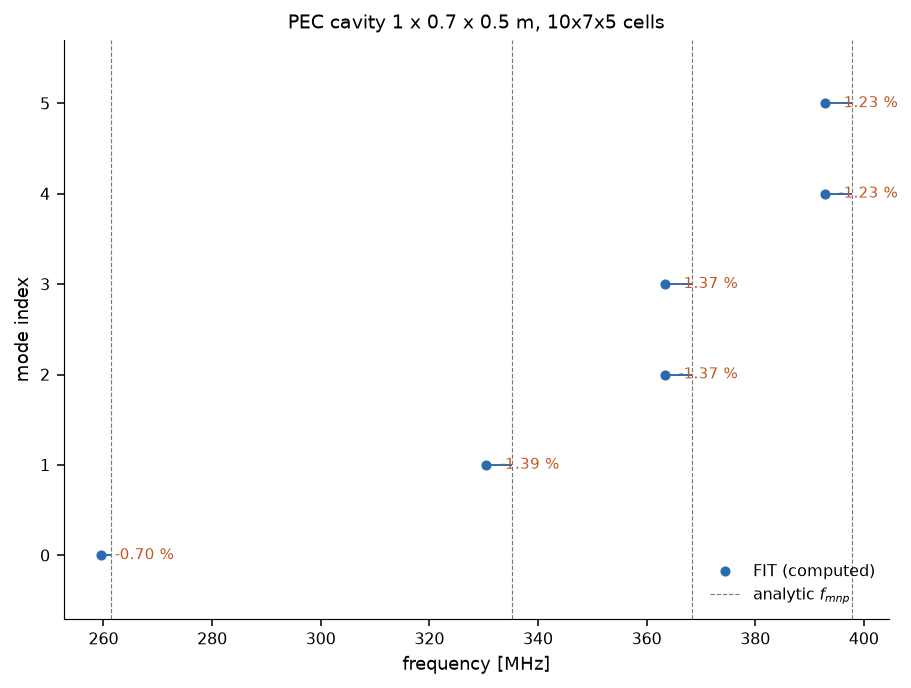
\includegraphics[width=0.78\textwidth]{../figures/cavity_spectrum.png}
  \caption{Resonances of the PEC box $1.0\times0.7\times0.5$ m on the $10\times7\times5$ grid, obtained by
  Fourier analysis of the $1500$-step ring-down that follows the drive. Computed frequencies are compared with
  the analytic modes of \eqref{eq:analytic}. The first six computed modes lie below their analytic counterparts,
  as a lumped material operator on a staggered grid must place them, and the two degenerate pairs are resolved as
  exactly equal pairs.}
  \label{fig:spectrum}
\end{figure}

Figure~\ref{fig:spectrum} is the frequency-domain output of a time-domain run: the field is stepped, the
ring-down is transformed, and the peaks of the transform are the resonances. That route to a spectrum is worth
having on its own, because it exercises the stepper rather than the eigensolver, and a mistake in the update
{\eqref{eq:leapfrog-h}--\eqref{eq:leapfrog-e}} would move the peaks. The six modes it finds are
$259.57$, $330.52$, $363.38$, $363.38$, $392.85$ and $392.85$ MHz against analytic values of $261.39$, $335.18$,
$368.42$, $368.42$, $397.74$ and $397.74$ MHz, a mean relative error of $1.213$\,\%, with the two degenerate
pairs reproduced to the last printed digit.

We deliberately do not tabulate those numbers again. The authoritative statement of the cavity spectrum is
Table~\ref{tab:cavity} and the order-of-convergence study is Table~\ref{tab:convergence}; both come from the
eigensolver of Section~\ref{sec:eigen}, which is the path that produces frequencies to a stated accuracy. What
Figure~\ref{fig:spectrum} adds is that the same spectrum is reachable from the time domain, that the extraction
is not doing anything delicate -- the peaks are far above the noise floor of a run whose energy is conserved to
rounding -- and that the two paths agree, which is a check on both.

The two pairs are degenerate because the box is not square in plan: the $363.38$ MHz and $392.85$ MHz modes each
come in a twofold set that the analytic count \eqref{eq:analytic} also produces, and their computed equality is
the symmetry of the discrete problem showing through. A solver that broke the pair apart by a fraction of a
percent would be telling us that its numbering or its stencil was not symmetric, so the printed pairs are a
sharper test than the mean error suggests.

\subsection{The field}
\label{sec:res-field}

\begin{figure}[H]
  \centering
  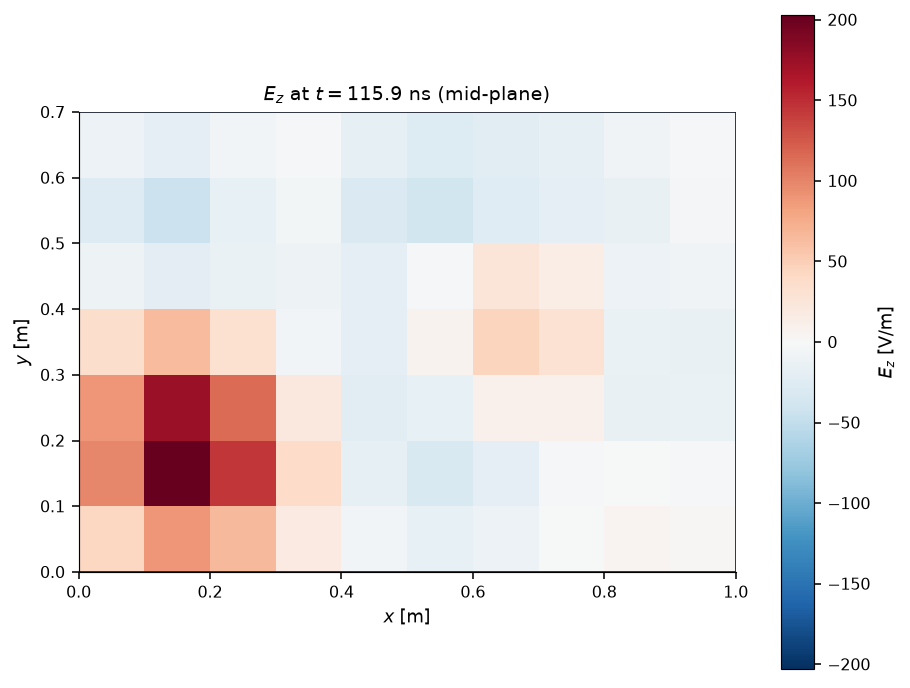
\includegraphics[width=0.72\textwidth]{../figures/cavity_field_z.png}
  \caption{The $z$ component of the electric field on the mid-plane of the cavity, taken at the moment the
  maximum field norm is reached during the drive. Sign changes across the box and the vanishing on the conducting
  walls are the features to look for: the pattern is the one the corresponding analytic mode predicts, with the
  nodal planes where they belong and the field tangential to the walls suppressed to zero.}
  \label{fig:field}
\end{figure}

Figure~\ref{fig:field} is the field map an engineer would ask for first, and it is the cheapest of the three to
read. It is a slice through the box at the instant of maximum field norm during the drive, so it shows the
excitation pattern rather than a single eigenvector -- the ring-down is a superposition, and a snapshot of a
superposition on a cut plane is honest about that. What the eye can check is qualitative but not soft: the sign
changes across the box are in the right places for the lowest modes of this box, and the field is zero on the six
walls to within the plotting resolution, which is the discrete counterpart of the boundary condition
\eqref{eq:leapfrog-pec}.

The slice is drawn by sampling the field on the nodes of the plane and interpolating from the edge-based unknowns,
which is the one piece of post-processing in the package that is not a plain reshape; it lives in
\texttt{viz.py} and it is the only place where a field component is moved from an edge to a point. Nothing in the
solver depends on it, and the figure is therefore evidence about the solution rather than evidence about the
pipeline that draws it.

\subsection{Energy in the same run}
\label{sec:res-energy}

\begin{figure}[H]
  \centering
  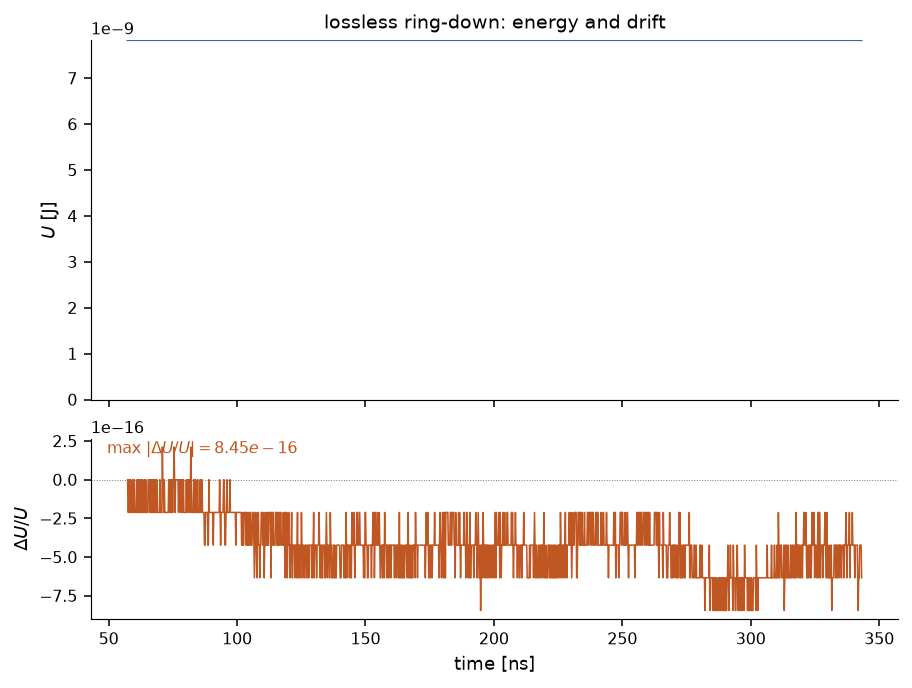
\includegraphics[width=0.85\textwidth]{../figures/energy_drift.png}
  \caption{Energy of the driven cavity run. Top: the invariant \eqref{eq:invariant} over the whole $1800$ steps,
  including the drive, on a linear scale on which the \SI{300}{} driven steps and the following
  \SI{343}{\nano\second} of ring-down are indistinguishable from a constant. Bottom: the relative drift on a
  logarithmic scale, which is where the interesting structure is -- the residual is at the level of a rounding
  floor, and it does not grow with step count.}
  \label{fig:energy}
\end{figure}

Figure~\ref{fig:energy} is the same run seen from the point of view of Section~\ref{sec:energy}. On a linear
scale the energy is a horizontal line: the drive injects power for $300$ steps, the source is switched off, and
the ring-down that follows neither gains nor loses energy at any scale a plot can show. The lower panel is the
same quantity on a logarithmic axis, and it is the informative one. The peak relative deviation over the recorded
portion is $8.451\times10^{-16}$, which is a few multiples of $\epsilon_{\mathrm{mach}}$ -- the rounding of a
double-precision sum of a few thousand positive terms, not a truncation error that a finer grid would reduce.

This is the strongest single statement in the report, and it is worth being precise about what it means. It is
not that the scheme conserves energy approximately, or that the drift is small enough not to matter. It is that
the quadratic form \eqref{eq:invariant}, evaluated on the staggered pair $(\mathbf{e}^{n},\mathbf{h}^{n-1/2})$
with its sign-indefinite cross term, is preserved to rounding by the update as implemented, on a run of $1800$
steps including a driven phase, in a cavity with conductor losses set to zero by construction. The comparison
against the three neighbouring candidate forms is in Table~\ref{tab:candidates} and is not repeated here; the
figure shows the winning candidate on a run long enough to make the point once, rather than the discrimination
that section already made.

\subsection{The time-domain checks}
\label{sec:res-time}

Two measurements in the suite are time-domain measurements, and both are quoted here because they are the only
quantitative checks on the stepper that do not involve a cavity.

The first is the conservation study of Table~\ref{tab:candidates}: a $12\times10\times8$ grid, random initial
fields, $500$ undriven steps, measured drift $1.298\times10^{-15}$ with the tolerance of the test set at $10^{-6}$
so that it asserts structure rather than a number. The same section records $8.45\times10^{-16}$ over $1500$ steps
and $1.669\times10^{-15}$ on a live run of the conservation test. We add only that these three values differ by a
factor of order two in the last digit and not in the exponent, which is the signature of a rounding floor sampled
at three points: there is no trend with step count to extrapolate, and no drift to blame on anything.

The second is the wave speed. On a $40\times6\times6$ grid with $h=0.02$ m, a broadband pulse whose nominal
wavelength spans about ten cells, and a probe ten cells downstream of the source, the front arrives at
$0.904\,c_0$ -- measured relative to the distance travelled and the elapsed time, with arrival defined as the
first sample above five per cent of the probe's peak. Section~\ref{sec:dispersion} derives the relation
\eqref{eq:phase} and shows that this number is what the formula predicts for a front whose leading edge sits at
about four cells per wavelength; the deficit is a second-order bias with the sign the theory gives it, it
vanishes as $h/\lambda\to0$, and it is neither an instability nor a symptom of a wrong operator. In the same
test, the field at the probe is exactly zero in the first three steps after the source is excited, which is the
causality check on a scheme that advances both fields at once.

\subsection{What this establishes, and what it does not}
\label{sec:res-scope}

It is worth separating the two, because the results above are strong and narrow at the same time.

What the results establish is the following. The discrete operators satisfy the identities of
Section~\ref{sec:theory} exactly, in integer arithmetic and independently of the mesh metric. The discrete
energy is conserved by the stepper to round-off over thousands of steps, which is a statement about the update
and not about the accuracy of its solution. The cavity spectrum converges at second order and lies within about
one per cent of the analytic box spectrum on the coarse grids used here, with the errors decreasing
at the rate Table~\ref{tab:convergence} measures. And a wavefront travels at a speed consistent with the
dispersion relation of the scheme, with the correct sign and the correct size.

What the results do not establish is anything about radiation. Every number in this section comes from a problem
whose boundary is a perfect conductor, so no field ever has to leave the domain, and the solver was never asked
to do the thing that an open-region problem demands: absorb an outgoing wave without reflecting it, and compute a
field at a distance. There is no absorbing boundary condition in the package, no near-to-far-field transform and
no port, and consequently there is no scattering result, no impedance and no $S$-parameter here. A cavity is the
easiest problem in computational electromagnetics precisely in this respect -- it is the one case where the
boundary condition costs nothing -- so the accuracy quoted above should be read as an accuracy about the
interior problem, on which every open-region result will later rest but none of which it can replace.

Closing that gap is the next milestone rather than a refinement of this one, and the acceptance test for it is
stated in terms of a quantity we cannot currently compute at all. Until a scatterer's bistatic radar cross
section has been compared with a Mie series, the honest summary of the present state is that the machinery is
verified and the physics it can address is still enclosed by walls.
